\chapter{Diseño e implementación del sistema de scripts}
\label{cap:diseñoImplentacion_scripts}

% Corregido 29/12/2023
% TODO:danielg: Revisar la introducción del capítulo

Como hemos visto en el capítulo \ref{cap:objetivos} el objetivo principal de este
proyecto es poder generar código en C a partir de un fichero ejecutable en su forma
de ensamblador. Para poder alcanzar este objetivo nos asistiremos con inteligencia
artificial de tal manera que podamos conseguir resultados óptimos. Para ello deberemos
de generar un \textit{dataset} que contenga los datos necesarios para poder entrenar
nuestro modelo.

Por ello, se ha diseñado un sistema de scripts que nos permitirá automatizar el proceso
de generar nuestro \textit{dataset}. Para el diseño de este sistema se han seguido los
siguientes criterios:

\begin{itemize}
    \item \textbf{Modularidad:} el sistema de scripts debe de ser modular, de tal manera
        que se puedan añadir nuevas funcionalidades de manera sencilla.
    \item \textbf{Mantenibilidad:} el sistema de scripts debe de ser mantenible, de tal
        manera que se puedan corregir errores o añadir nuevas funcionalidades de manera
        sencilla.
    \item \textbf{Portable:} el sistema de scripts debe de ser portable, de tal manera
        que se pueda ejecutar en cualquier sistema operativo.
\end{itemize}

\section{Diseño del sistema de scripts}
\label{sec:diseño_sistema_scripts}

\newpage
\paperwidth=\pdfpageheight
\paperheight=\pdfpagewidth
\pdfpageheight=\paperheight
\pdfpagewidth=\paperwidth
\headwidth=\textheight

\subsection{Diagrama de clases}
\label{subsec:diagrama_clases}

% TODO:danielg: Comprobar que el UML corresponde al diseño final

\begin{figure}[H]
    \begin{center}
        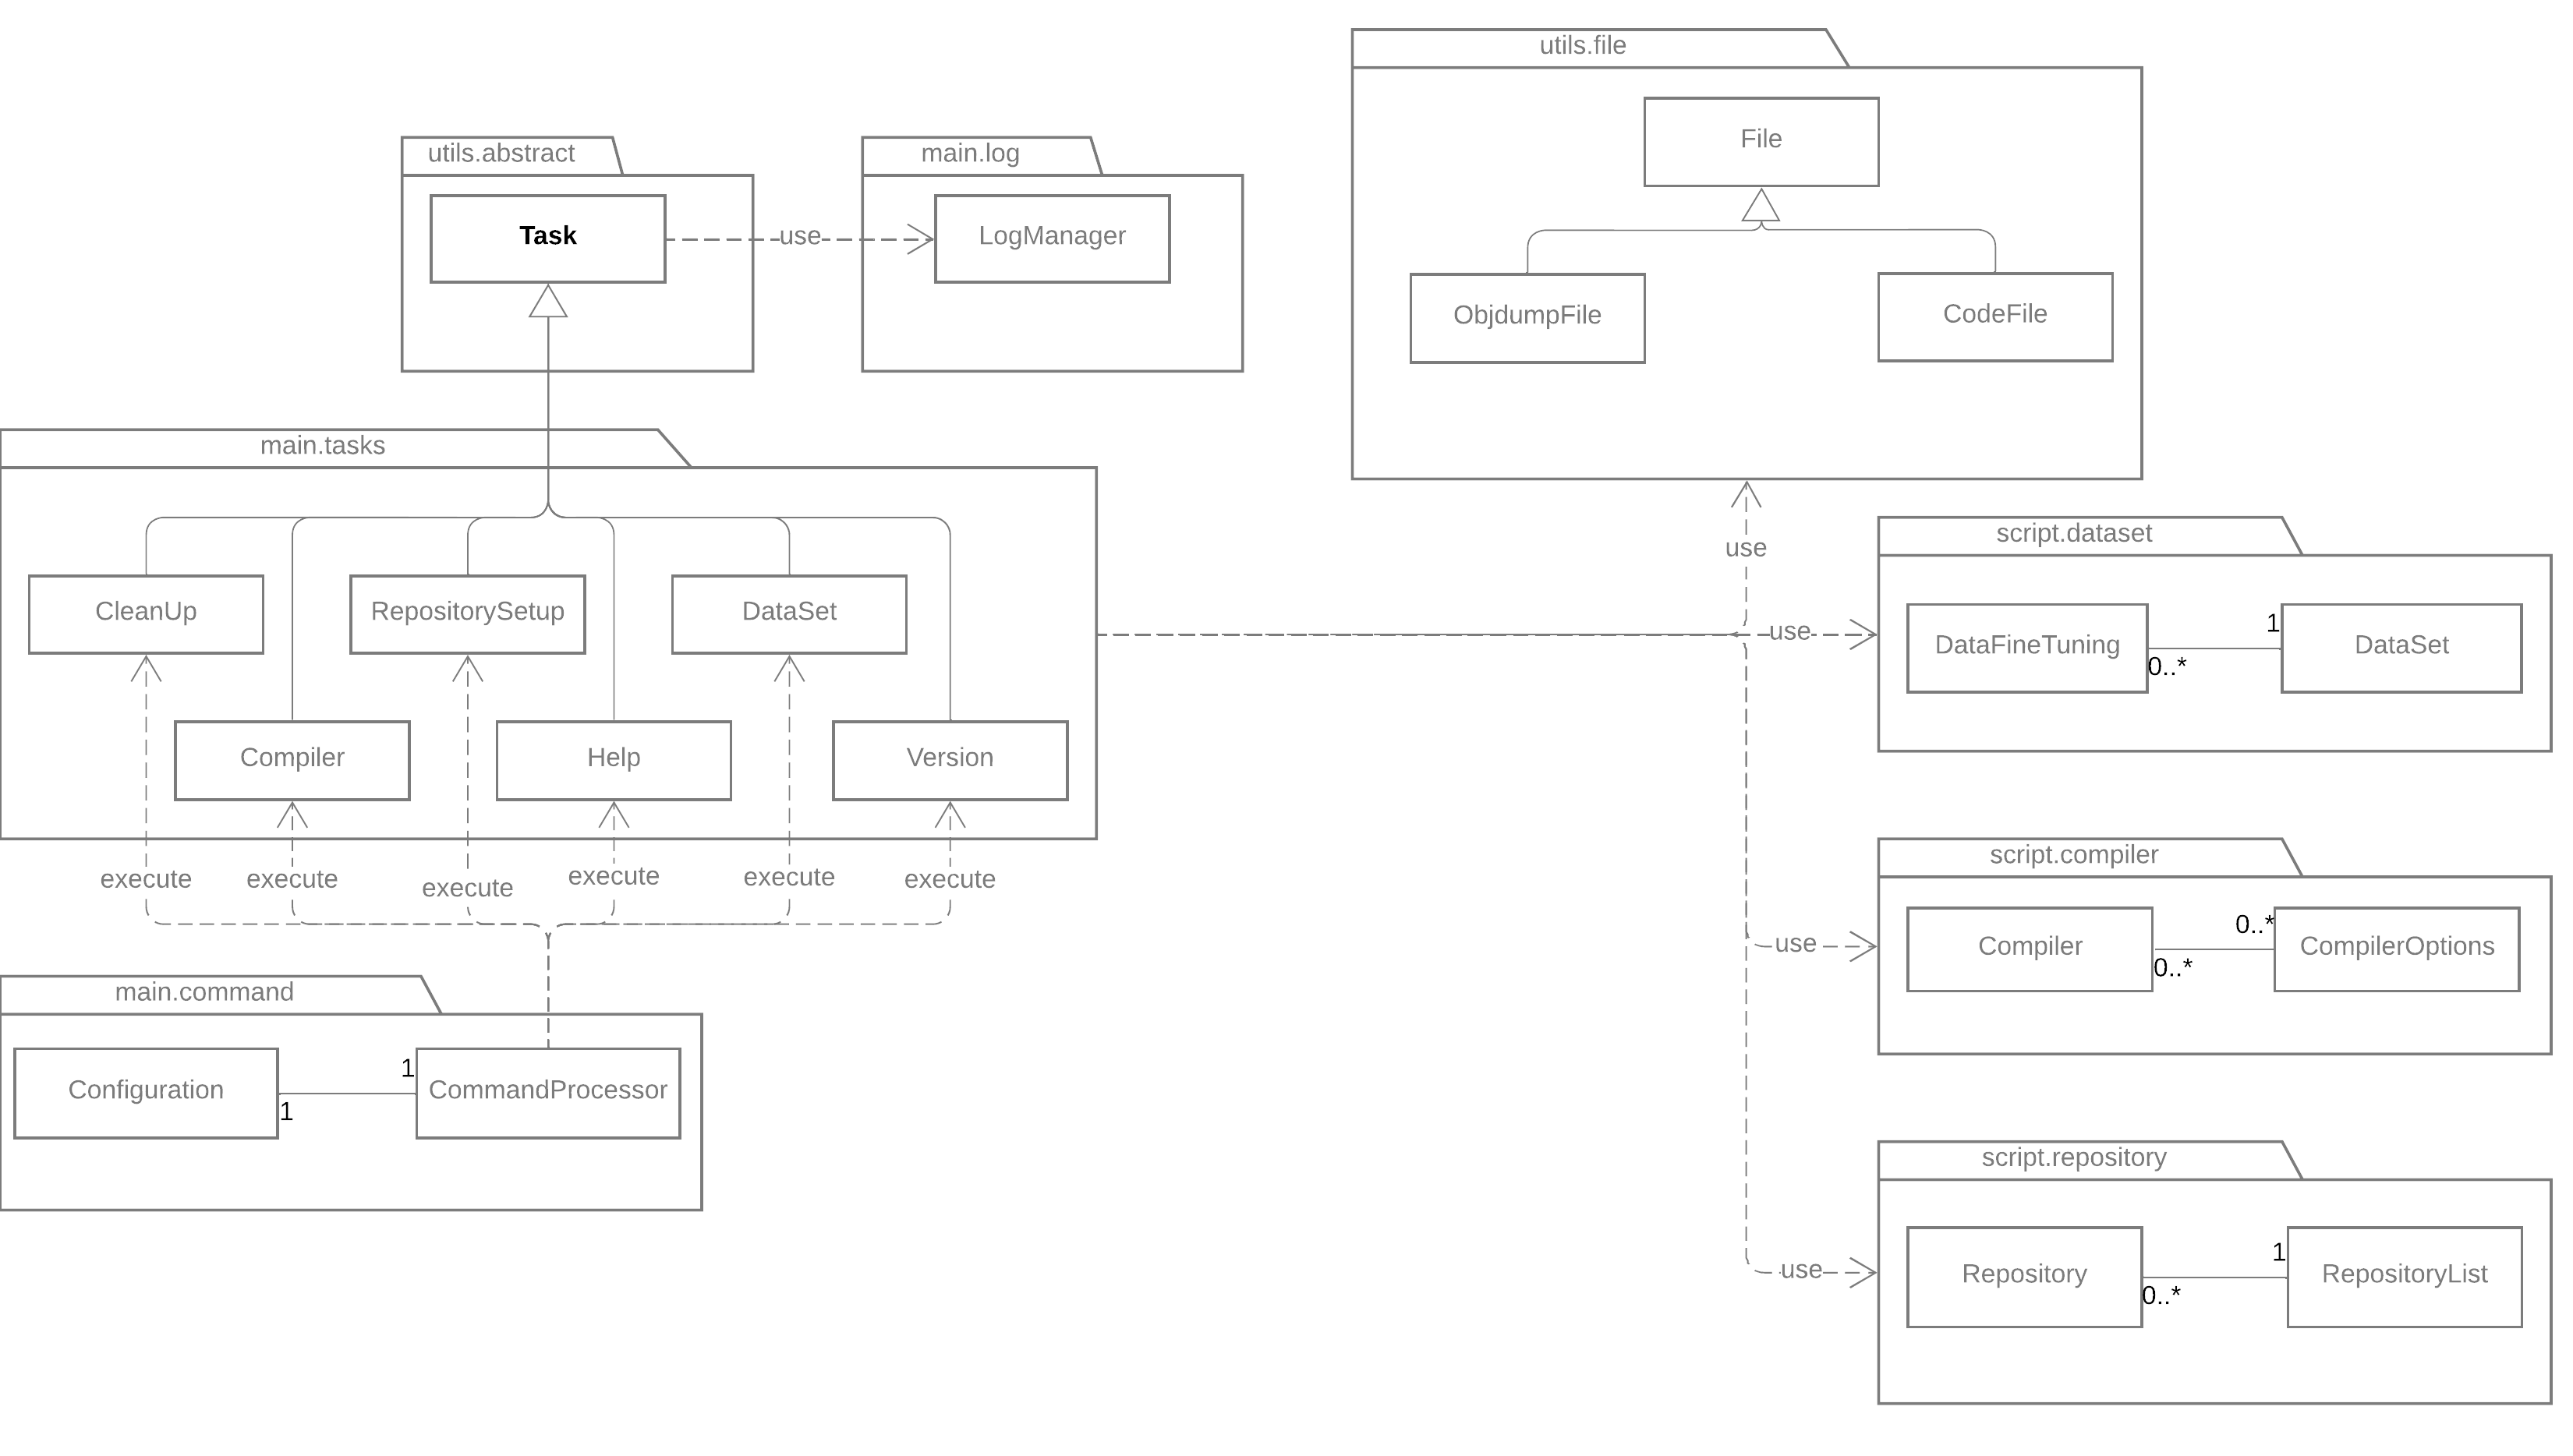
\includegraphics[scale=0.2]{figuras/Capitulo_XX/UML_Script.png}
    \end{center}
    \caption[Diagrama de clases del sistema de scripts]{Diagrama de clases del sistema de scripts (Elaboración propia)}
    \label{fig:UML_Script}
\end{figure}\

\newpage
\paperwidth=\pdfpageheight
\paperheight=\pdfpagewidth
\pdfpageheight=\paperheight
\pdfpagewidth=\paperwidth
\headwidth=\textwidth

\section{Implementación del sistema de scripts}
\label{sec:implementacion_sistema_scripts}

